\documentclass[10pt,xcolor=table]{beamer}
\usetheme{Warsaw}
%\usepackage[T1]{fontenc}
%\usepackage[utf8]{inputenc}
\usepackage{polski}
\usepackage{amsmath}
\usepackage{amsfonts}
\usepackage{amssymb}
\usepackage{amsbsy}
\usepackage{graphicx}
\usepackage{booktabs}
\usepackage{makecell}
\usepackage{pifont}
\usepackage{tikz}
\usetikzlibrary{positioning,arrows.meta,shapes.geometric}
\tikzset{
  box/.style={draw=blue!50!black, fill=blue!8, rounded corners=2pt, align=center,
              minimum height=1cm, minimum width=1.7cm, font=\scriptsize},
  ours/.style={box, fill=orange!20, draw=orange!70!black},
  file/.style={box, fill=gray!10, draw=gray!60!black},
  db/.style={cylinder, shape border rotate=90, aspect=0.25, draw=blue!50!black,
             fill=blue!8, align=center, minimum width=1.6cm, minimum height=1cm, font=\scriptsize},
  arr/.style={-{Stealth[length=2mm]}, thick, draw=black!70},
  lbl/.style={font=\tiny, midway, inner sep=1pt},
}
\newcommand{\cmark}{{\color{green!60!black}\ding{51}}}
\newcommand{\xmark}{{\color{red!70!black}\ding{55}}}
\newcommand{\pmark}{{\color{orange}$\sim$}}
\renewcommand{\theadfont}{\bfseries}
\author{Dawid Pągowski \& Bartłomiej Łokaj \& Paweł Świderski}
\title[\insertframenumber/\inserttotalframenumber]{
	Analizator logów Apache
}
%\setbeamercovered{transparent} 
%\setbeamertemplate{navigation symbols}{} https://www.overleaf.com/project/6161cfd1849aaa13376b82eb
\logo{
\includegraphics[height=1cm]{media/logoMS.png}} 
\institute{
	
\includegraphics[height=1cm]{media/logo.jpg}\\
	Wydział Matematyki Stosowanej
}
\date{\today}  

\begin{document}
\begin{frame}
	\titlepage
\end{frame}
\section*{Agenda}
\begin{frame}
    \frametitle{Agenda}
	\tableofcontents
\end{frame}
\section{Założenia}
\begin{frame}
    \frametitle{Cel}
    \begin{block}{Cel}
    \begin{itemize}
        \item Analiza logów serwera Apache w celu wykrywania podejrzanego ruchu
        \item Zapisywanie podejrzanych zdarzeń w bazie
        \item Efekt wow: aktywne blokowanie hostów na podstawie pojedynczych żądań w serwerze Apache 
    \end{itemize}
    \end{block}  
\end{frame}
\section{Uwarunkowania prawne}
\begin{frame}
    \frametitle{Uwarunkowania prawne}
    \begin{block}{Uwarunkowania prawne}
    \begin{itemize}
        \item Całe rozwiązanie hostowane lokalnie, nic nie wychodzi poza infrastrukturę 
        \item Adresy IP to dane osobowe. Dane przechowywane na podstawie prawnie uzasadnionego interesu administratora (art. 6 ust. 1 lit. f RODO)
        \item Zdarzenia mają ograniczony czas przechowywania
    \end{itemize}
    \end{block}  
\end{frame}
\section{Organizacja projektu}
\begin{frame}
    \frametitle{Organizacja projektu}
    \begin{block}{Organizacja projektu}
    \begin{itemize}
        \item Tracker zadań: self-hostowany, modyfikowany Plane Community
        \item Repozytorium git: na GitHubie. Pull-requesty+CI/CD
    \end{itemize}
    \end{block}  
\end{frame}
\subsection{Podział pracy}
\begin{frame}
    \frametitle{Podział pracy}
    \begin{block}{Podział pracy}
    \begin{itemize}
        \item Bartłomiej Łokaj: backend ASP.NET Core, silnik wykrywania niebezpiecznych żądań wykorzystujący sztuczną inteligencję
        \item Paweł Świderski: frontend React
        \item Dawid Pągowski: "lead", integracja z serwerem Apache, wdrażanie rozwiązań, silnik parsowania logów do obiektów C\#, zarządzanie serwerem Apache
    \end{itemize}
    \end{block}  
\end{frame}
\subsection{Główne fazy}
\begin{frame}
    \frametitle{Główne fazy}
    \begin{block}{Główne fazy}
    \begin{itemize}
        \item Prototyp: stawianie serwera Apache w Internecie w celu zbierania logów, szkielet modułu Apache oraz parsera, model wykrywania niebezpiecznych zdarzeń, mockup frontendu
        \item MVP: łączenie komponentów w działającą całość, działający tryb analizy, reguły statyczne, testy E2E oraz wydajnościowe
        \item Wersja końcowa: tryb blokady (działający moduł Apache), strojenie modelu na zebranych danych (+ ewentualne tworzenie datasetu atakując nasz własny serwer), zarządzanie regułami z aplikacji React, dokumentacja
    \end{itemize}
    \end{block}  
\end{frame}
\section{Porównanie z innymi narzędziami}
\begin{frame}
  \frametitle{Porównanie z innymi narzędziami}
  \centering
  \scriptsize
  \setlength{\tabcolsep}{5pt}
  \renewcommand{\arraystretch}{1.25}
  \begin{tabular}{l l c c c c}
    \toprule
    \thead{Narzędzie} & \thead{Typ} & \thead{Wykrywanie\\ataków} & \thead{Baza\\zdarzeń}
      & \thead{Aktywne\\blokowanie} & \thead{AI} \\
    \midrule
    GoAccess          & statystyki ruchu & \xmark & \xmark & \xmark & \xmark \\
    AWStats           & statystyki ruchu & \xmark & \xmark & \xmark & \xmark \\
    Fail2ban          & reguły regex     & \pmark & \pmark & \cmark{} (IP) & \xmark \\
    ModSecurity + CRS & WAF w Apache     & \cmark & \xmark & \cmark{} (żądania) & \xmark \\
    Wazuh / ELK       & SIEM             & \cmark & \cmark & \cmark{} (IP) & \pmark \\
    \midrule
    \rowcolor{blue!8}
    \textbf{Nasz analizator} & reguły + AI & \cmark & \cmark & \cmark{} (IP + żądania) & \cmark \\
    \bottomrule
  \end{tabular}

  \vspace{1.5ex}
  {\tiny \cmark~tak \qquad \pmark~częściowo \qquad \xmark~nie}
\end{frame}
\section{Wstępny mechanizm działania}
\subsection{Tryb analizy}
\begin{frame}
    \frametitle{Mechanizm działania -- tryb analizy}
    \begin{block}{Tryb analizy}
    \begin{itemize}
        \item Apache zapisuje logi do pliku wedle konfigurowalnego formatu
        \item Format zawiera źródłowe adresy IP, ścieżkę dostępu, metody HTTP
        \item Pasywny reader odczytuje logi, wysyła do backendu
        \item Backend kategoryzuje czy dane żądanie było podejrzane czy nie za pomocą sztucznej inteligencji oraz reguł statycznych
    \end{itemize}
    \end{block}  
\end{frame}
\begin{frame}
  \frametitle{Schemat -- tryb analizy}
  \centering
  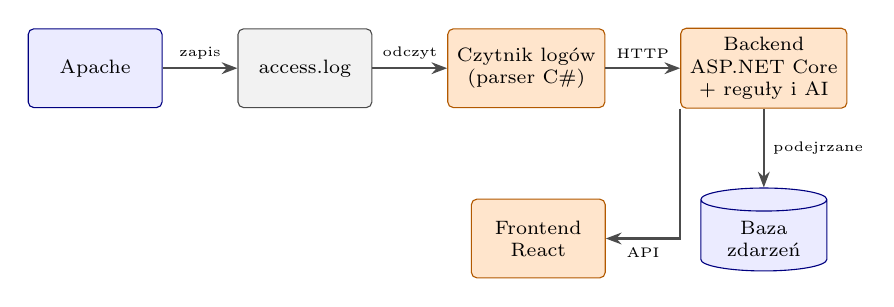
\begin{tikzpicture}[node distance=0.95cm]
    \node[box]  (apache)  {Apache};
    \node[file, right=of apache] (log) {access.log};
    \node[ours, right=of log]    (reader) {Czytnik logów\\(parser C\#)};
    \node[ours, right=of reader] (backend) {Backend\\ASP.NET Core\\+ reguły i AI};
    \node[db,   below=1cm of backend] (db) {Baza\\zdarzeń};
    \node[ours, left=1.2cm of db]   (front) {Frontend\\React};

    \draw[arr] (apache) -- node[lbl, above=2pt] {zapis} (log);
    \draw[arr] (log) -- node[lbl, above=2pt] {odczyt} (reader);
    \draw[arr] (reader) -- node[lbl, above=2pt] {HTTP} (backend);
    \draw[arr] (backend) -- node[lbl, right=2pt] {podejrzane} (db);
    \draw[arr] (backend.south west) |- node[lbl, pos=0.75, below=2pt] {API} (front);
  \end{tikzpicture}

  \vspace{2ex}
  {\scriptsize Analiza po fakcie -- żądanie zostało już obsłużone, zdarzenie trafia do bazy.}
\end{frame}
\subsection{Tryb blokady}
\begin{frame}
    \frametitle{Mechanizm działania -- tryb blokady}
    \begin{block}{Tryb blokady}
    \begin{itemize}
        \item Tryb blokady podejrzanych żądań nie może odbywać się na podstawie samych logów. Logi zawierają już zakończone żądania.
        \item Na potrzeby trybu blokady zostanie stworzony lekki moduł Apache przekazujący przychodzące żądania do backendu
        \item Backend kategoryzuje czy dane żądanie było podejrzane czy nie za pomocą sztucznej inteligencji oraz reguł statycznych, tak samo jak w przypadku trybu analizy
        \item Jeżeli żądanie zostanie uznane za bezpieczne, moduł przepuszcza żądanie. W innym wypadku zostaje odrzucone.
        \item Problemem mogą być opóźnienia oraz padnięty backend. Rozwiązaniem byłaby optymalizacja modelu + tryb fail-open, który przepuszcza żądania, gdy backend nie odpowiada.
    \end{itemize}
    \end{block}  
\end{frame}
\begin{frame}
  \frametitle{Schemat -- tryb blokady}
  \centering
  \begin{tikzpicture}[node distance=0.9cm]
    \node[file] (client) {Klient};
    \node[box, right=of client, minimum width=3cm, minimum height=1.6cm] (apache) {};
    \node[font=\scriptsize, anchor=north] at (apache.north) {Apache};
    \node[ours, minimum width=2.4cm, minimum height=0.6cm, anchor=south]
         at ([yshift=3pt]apache.south) (mod) {nasz moduł};
    \node[ours, right=2.1cm of apache] (backend) {Backend\\ASP.NET Core\\+ reguły i AI};
    \node[box, below=1.1cm of apache] (app) {Aplikacja\\(strona)};
    \node[file, fill=red!10, draw=red!60!black, left=of app] (deny) {403\\Forbidden};

    \draw[arr] (client) -- node[lbl, above=2pt] {żądanie} (apache);
    \draw[arr] ([yshift=4pt]mod.east) -- node[lbl, above=2pt] {treść żądania} ([yshift=-9pt]backend.west);
    \draw[arr] ([yshift=-14pt]backend.west) -- node[lbl, below=2pt] {werdykt} ([yshift=-6pt]mod.east);
    \draw[arr, green!50!black] (mod) -- node[lbl, right=2pt] {bezpieczne} (app);
    \draw[arr, red!70!black] (mod.south west) -- node[lbl, above left=0pt] {podejrzane} (deny);
  \end{tikzpicture}

  \vspace{2ex}
  {\scriptsize Brak odpowiedzi backendu w limicie czasu $\Rightarrow$ fail-open (żądanie przepuszczone).}
\end{frame}
\subsection{Reguły statyczne}
\begin{frame}
  \frametitle{Reguły statyczne (bez AI)}
  \begin{block}{Reguły statyczne}
  \begin{itemize}
    \item Proste reguły (wzorce, regex) definiowane przez administratora, sprawdzane przed modelem AI
    \item Przykłady:
    \begin{itemize}
      \item LFI / path traversal: \texttt{../../etc/passwd}, \texttt{\%2e\%2e\%2f}
      \item Dostęp do wrażliwych plików: \texttt{/.env}, \texttt{/.git/config}
      \item Znane skanery w User-Agent: \texttt{sqlmap}, \texttt{nikto}
    \end{itemize}
    \item Dopasowanie reguły oznacza natychmiastowy werdykt, bez odpytywania modelu
    \item Zalety: deterministyczne, szybkie, łatwe do wyjaśnienia; odciążają model i zmniejszają opóźnienia w trybie blokady
  \end{itemize}
  \end{block}
\end{frame}
\section{Otwarte kwestie}
\begin{frame}
  \frametitle{Otwarte kwestie}
  \begin{itemize}
    \item Jaki model: lekki klasyfikator (jev, kev, inny decyzyjny) czy większy model (LLM, większa ilość parametrów)?
    \item Dane treningowe: jak oznaczać ruch normalny i złośliwy z własnego serwera?
    \item Tryb blokady: jakie opóźnienie jest akceptowalne i jaki ustawić timeout?
  \end{itemize}
\end{frame}
\end{document}
